%\documentclass[11pt,a4paper]{article}
\documentclass[11pt
  , a4paper
  , article
  , oneside
%  , twoside
%  , draft
]{memoir}

\usepackage{control}
\usepackage[numbers]{natbib}


\begin{document}

\newcommand{\technumber}{
  RAON Control-Document Series\\
  Revision : v0.1,   Release : 2016. 01. 15}
\title{\textbf{LLRF용 EPICS IOC 설치 로그}}



\author{남승희\thanks{namsh@ibs.re.kr} \\
  Control Group \\
  Rare Isotope Science Project\\
  Institute for Basic Science\\
  Daejeon, South Korea
}

\date{\today}

\renewcommand{\maketitlehooka}{\begin{flushright}\textsf{\technumber}\end{flushright}}
%\renewcommand{\maketitlehookb}{\centering\textsf{\subtitle}}
%\renewcommand{\maketitlehookc}{C}
%\renewcommand{\maketitlehookd}{D}

\maketitle





\chapter{Debian Linux 설치}
LLRF용 EPICS server의 OS는 Debian7 Linux 32bit를 사용하며 자세한 내용은 아래와 같다.
\begin{lstlisting}[style=termstyle]
root@LLRF-Intech:~# uname -a
Linux LLRF-Intech 3.2.0-4-686-pae #1 SMP Debian 3.2.73-2+deb7u2 i686 GNU/Linux
\end{lstlisting}
\section{설치}
설치를 위해서는 위에서 언급한 데비안 리눅스 버전이 필요하다. 마이너한 버전의 차이는 상관이 없을것으로 보이나 메이저한 버전의 차이는 시스템 라이브러리쪽에서 문제가 발생할수도 있으므로도 가급적 Debian7 Linux 32bit를 사용하여 설치하길 바란다. OS 설치는 대부분의 사람이 할 수 있으므로 생략하고 주의 사항 몇가지만 언급한다.
\subsection{Machine Name}
업체에서 개발된 LLRF용 EPICS IOC는 LLRF-Intech이라는 machine name을 사용하므로 별다른 이유가 있지 않으면 설치시 LLRF-Intech을 machine name으로 지정한다.
\subsection{User Name}
업체에서 개발된 LLRF용 EPICS IOC는 llrf라는 user name을 사용하므로 user name은 꼭 llrf를 사용한다. llrf라는 이름을 사용하지 않으면 LLRF용 EPICS IOC를 사용할때 많은 경로 에러가 발생한다. 설치가 끝나면 터미널상에서 다음과 같이 username@machinename을 확인할 수 있다.
\begin{lstlisting}[style=termstyle]
llrf@LLRF-Intech:~$
\end{lstlisting}
\section{네트워크설정}
LLRF는 192.168.0.177의 IP를 사용하고 게이트웨이는 192.168.0.1을 사용한다. LLRF와의 통신을 위해서 컴퓨터는 고정 IP를 사용한다.\\
IP : 192.168.0.100\\
Netmask : 255.255.255.0\\
Gateway : 192.168.0.1\\
\begin{figure}[h!]
	\centering
	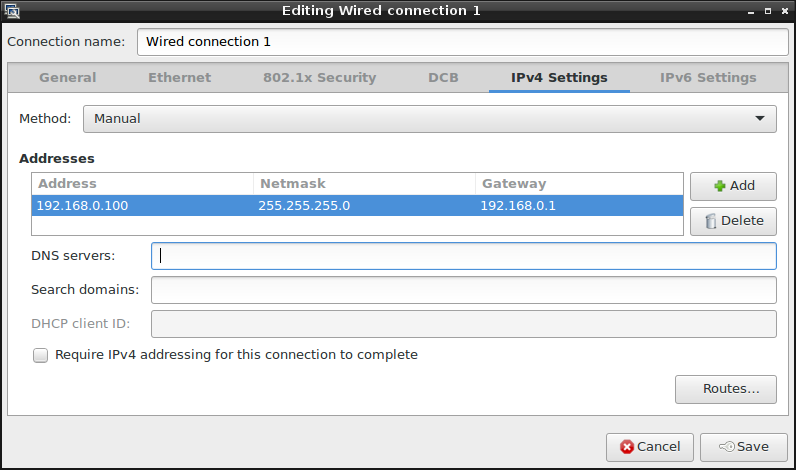
\includegraphics[width=0.6\textwidth, height=0.6\textwidth]{./images/4.png}
	\caption{IP설정}
\end{figure}
\chapter{EPICS 및 IOC 설치}
EPICS는 시스템 아키텍쳐가 같으면 복사하여 사용해도 상관 없으므로 EPICS 및 IOC를 복사하여 사용한다.
\section{EPICS를 위한 시스템 패키지 설치}
EPICS와 IOC는 복사를 하지만 업체에서 개발된 IOC는 EPICS base 부분과 synApp 부분을 사용하므로로 EPICS 및 synApp 구동에 필요한 패키지는 설치해 주어야한다. 필요 패키지는 다음과 같다.
\begin{itemize}
	\item build-essential
	\item libreadline-dev
	\item re2c
	\item python-dev
	\item libnetcdf-dev
	\item libhdf5-dev
	\item libnexus0-dev
	\item libpng12-0-dev
	\item libbz2-dev
	\item libxml2-dev
	\item libusb-dev
\end{itemize}
위의 패키지는 아래와 같이 설치하면된다.
\begin{lstlisting}[style=termstyle]
 llrf@LLRF-Intech:~$ su
 Password: 
 su: Authentication failure
 llrf@LLRF-Intech:~$ su
 Password: 
 root@LLRF-Intech:/home/llrf# aptitude install build-essential libreadline-dev re2c python-dev libnetcdf-dev libhdf5-dev libnexus0-dev libpng12-0-dev libbz2-dev libxml2-dev libusb-dev
\end{lstlisting}
\section{EPICS 및 IOC 복사}
EPICS 및 IOC와 IOC를 위한 라이브러리리들은 지정된 위치에 복사하여 사용한다. EPICS 및 IOC를 위한 파일들은 다음과 같다.
\begin{figure}[h!]
	\centering
	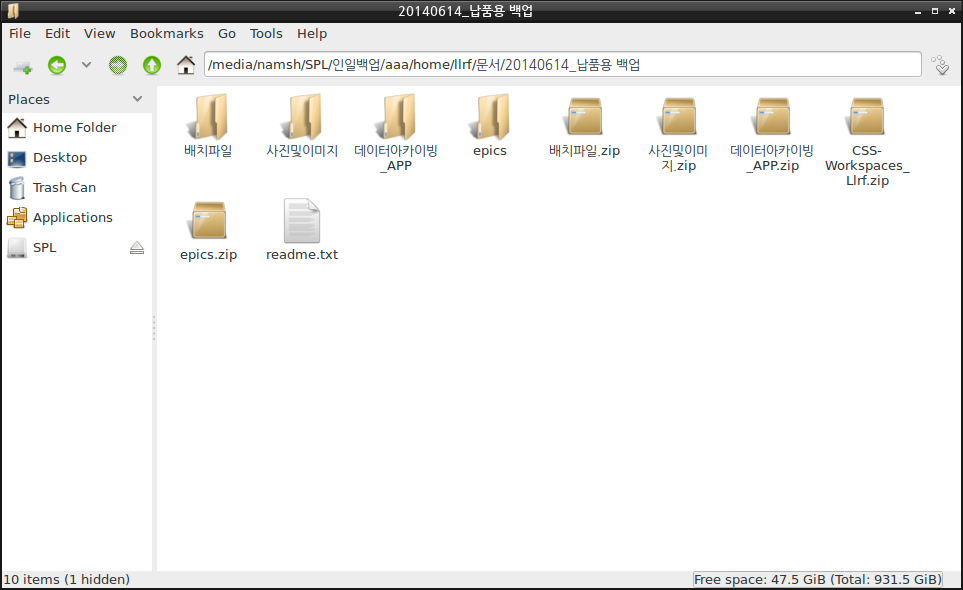
\includegraphics[width=0.6\textwidth, height=0.3\textwidth]{./images/1.png}
	\caption{20140614\_납품용백업 파일}
\end{figure}

이 밖에도 몇가지 파일이 필요하지만 나중에 언급하겠다. 복사가 안된다면 루트 권한으로 실행 하기를 바란다.
\subsection{epics 폴더 복사}
남품용백업 파일의 epics 폴더는 /usr/local로 복사한뒤 루트권한으로 epics 폴더에 권한을 설정한다.
\begin{lstlisting}[style=termstyle]
llrf@LLRF-Intech:/usr/local$ su
Password: 
root@LLRF-Intech:/usr/local# chmod -R 755 epics
\end{lstlisting}
\subsection{배치파일 복사}
배치파일 폴더 안에는 다음과 같은 파일이 있으며 이 파일들을 /home/llrf/에 복사한다.
\begin{figure}[h!]
		\centering
		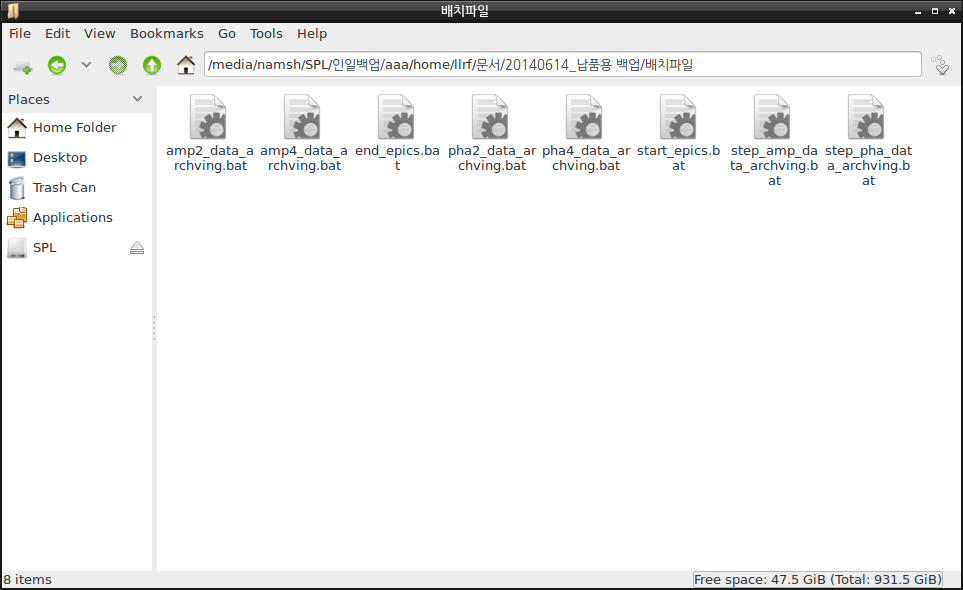
\includegraphics[width=0.6\textwidth, height=0.3\textwidth]{./images/2.png}
		\caption{배치파일}
\end{figure}
\subsection{DADA 폴더 복사}
데이터아카이빙\_APP의폴더 안의 DATA 폴더를 /home/llrf에 복사한다. 유저가 사용할수 있도록 루트 권한으로 DATA 폴더 안의 filetest 파일의 권한을 설정한다.
\begin{lstlisting}[style=termstyle]
llrf@LLRF-Intech:~/DATA$ su
Password: 
root@LLRF-Intech:/home/llrf/DATA# chmod 755 filetest
\end{lstlisting}
\subsection{CSS-Workspace\_Llrf.zip}
CSS-Workspace\_Llrf.zip의 압축을 해제하고 폴더를 살펴보면 CSS 실행을 위한 opi가 있다. 이 폴더는 편한곳에 복사한뒤 CSS 실행시 workspace를 복사한 곳으로 지정하면 된다. 
\subsection{이 밖에 필요한 파일}
\begin{itemize}
	\item /usr/bin의 caget, cainfo, camonitor, caput, caRepeater, casw 파일\\
	\begin{figure}[h!]
		\centering
		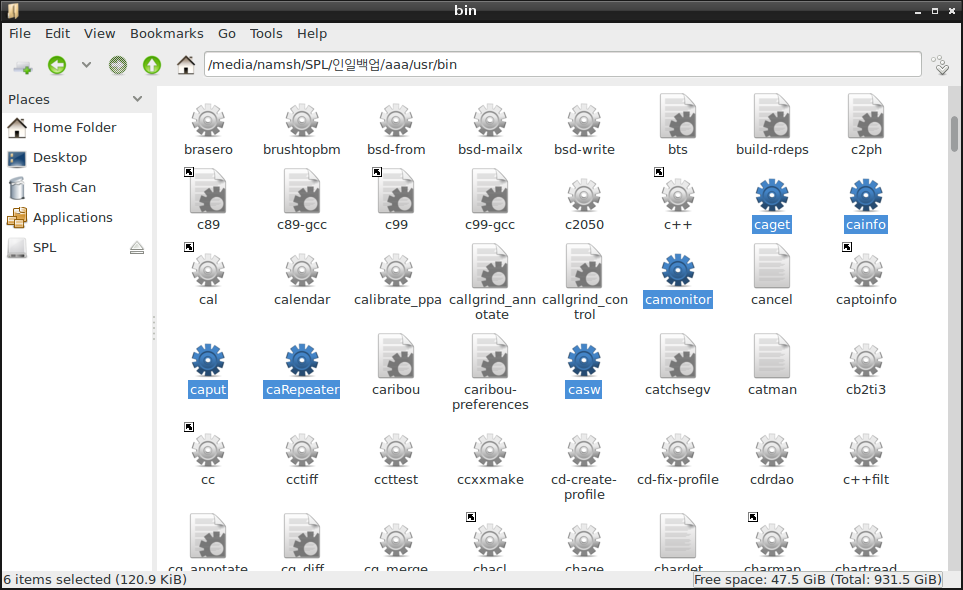
\includegraphics[width=0.85\textwidth, height=0.6\textwidth]{./images/3.png}
		\caption{/usr/bin의 필요파일}
	\end{figure}
	위의 파일들을 ca command를 사용하기 위해서 내컴퓨터의 /usr/bin에 복사한다.
	\item /usr/lib의 epics 폴더와 libca.so.3.14.12.3, libCom.so.3.14.12.3 등 lib*.3.14.12.3 라이브러리 파일 : 현재 IOC 작동중 위 두개의 라이브러리만 필요로 하지만 차후 다른 기능을 사용할때 lib*.3.14.12.3 라이브러리를 필요로 할것으로 보인다. 복사뒤 라이브러리 파일에 권한을 준다.
	\begin{lstlisting}[style=termstyle]
	llrf@LLRF-Intech:/usr/lib$ su
	Password: 
	root@LLRF-Intech:/usr/lib# chmod 755 libca.so.3.14.12.3 libCom.so.3.14.12.3
\end{lstlisting}
\item CSS-BOY : 업체에서 opi를 css-boy를 사용하여 만들었기 때문에 css-boy를 사용한다. /usr/local의 css-boy를 내 컴퓨터의 /usr/local로 복사한다. 편한 css의 사용을 위해서 /home/llrf의 css 파일을 내컴퓨터의 /home/llrf에 복사하여 쓰거나 아래와 같이 링크를 걸어서 사용한다.
	\begin{lstlisting}[style=termstyle]
	llrf@LLRF-Intech:~$ su
	Password: 
	root@LLRF-Intech:/home/llrf# ln -s /usr/local/CSS-BOY/CSS_3.2.14/css
\end{lstlisting}
\end{itemize}
\chapter{EPICS IOC사용}
\section{터미널 내에서 EPICS 실행}
터미널에서 EPICS IOC 실행은 ./start\_epics.bat로 하고 실행 내용은 아래와 같다.
\begin{lstlisting}[style=termstyle]
llrf@LLRF-Intech:~$ ./start_epics.bat 
< envPaths
epicsEnvSet("ARCH","linux-x86")
epicsEnvSet("IOC","iocTest")
epicsEnvSet("TOP","/usr/local/epics/modules/synApps_5_7/support/modbus-2-4")
epicsEnvSet("SUPPORT","/usr/local/epics/modules/synApps_5_7/support")
epicsEnvSet("AUTOSAVE","/usr/local/epics/modules/synApps_5_7/support/autosave-5-1")
epicsEnvSet("ASYN","/usr/local/epics/modules/synApps_5_7/support/asyn-4-21")
epicsEnvSet("SSCAN","/usr/local/epics/modules/synApps_5_7/support/sscan-2-9")
epicsEnvSet("EPICS_BASE","/usr/local/epics/base")
#< Koyo1.cmd
< Koyo2.cmd
# Koyo2.cmd
dbLoadDatabase("../../dbd/modbus.dbd")
modbus_registerRecordDeviceDriver(pdbbase)
# Use the followi	ng commands for TCP/IP
#drvAsynIPPortConfigure(const char *portName,
#                       const char *hostInfo,
#                       unsigned int priority,
#                       int noAutoConnect,
#                       int noProcessEos);
#drvAsynIPPortConfigure("Koyo2","192.168.0.83:502",0,0,1)
#drvAsynIPPortConfigure("Koyo2","192.168.0.33:502",0,0,1)
drvAsynIPPortConfigure("Koyo2","192.168.0.177:502",0,0,1)
#modbusInterposeConfig(const char *portName,
#                      modbusLinkType linkType,
#                      int timeoutMsec, 
#                      int writeDelayMsec)
modbusInterposeConfig("Koyo2",0,2000,0)
#modbusInterposeConfig("Koyo2",0,2000,60)
# NOTE: We use octal numbers for the start address and length (leading zeros)
#       to be consistent with the PLC nomenclature.  This is optional, decimal
#       numbers (no leading zero) or hex numbers can also be used.
#       In these examples we are using slave address 0 (number after "Koyo2").
# The DL205 has word access to the V3000 memory at Modbus offset 3000 (octal)
drvModbusAsynConfigure("K2_V3000_In_Word1",   "Koyo2",    0, 3,  2001,  2,   8,  1,    "Koyo")
drvModbusAsynConfigure("K2_V3000_In_Word3",   "Koyo2",    0, 3,  2003,  2,   8,  1,    "Koyo")
#20140522 :portname,tcpportname,slaveaddress,modbusfunction,modbusstartaddress,modbuslength,datatype,pollmsec,plctype
#drvModbusAsynConfigure("K2_V3000_In_Word",   "Koyo2",    0, 3,  2000,  8,   8,  1,    "Koyo")
2016/01/15 18:47:42.002 drvModbusAsynConfigure("K2_V3000_In_Word5",   "Koyo2",    0, 3,  2005,  2,   8,  1,    "Koyo")
drvModbusAsyn::doModbusIO port K2_V3000_In_Word1 error calling writeRead, error=asynManager::queueLockPort queueRequest failed: port Koyo2 not connected, nwrite=2/6, nread=4
2016/01/15 18:47:42.002 drvModbusAsynConfigure("K2_V3000_In_Word7",   "Koyo2",    0, 3,  2007,  2,   8,  1,    "Koyo")
drvModbusAsyn::doModbusIO port K2_V3000_In_Word3 error calling writeRead, error=asynManager::queueLockPort queueRequest failed: port Koyo2 not connected, nwrite=2/6, nread=4
2016/01/15 18:47:42.002 drvModbusAsyn::doModbusIO port K2_V3000_In_Word5 error calling writeRead, error=asynManager::queueLockPort queueRequest failed: port Koyo2 not connected, nwrite=2/6, nread=4
drvModbusAsynConfigure("K2_V3000_In_Word8",   "Koyo2",    0, 3,  2100,  2,   8,  1,    "Koyo")
2016/01/15 18:47:42.002 drvModbusAsyn::doModbusIO port K2_V3000_In_Word7 error calling writeRead, error=asynManager::queueLockPort queueRequest failed: port Koyo2 not connected, nwrite=2/6, nread=4
drvModbusAsynConfigure("K2_V3000_In_Word9",   "Koyo2",    0, 3,  2101,  2,   8,  1,    "Koyo")
................
\end{lstlisting}
이때 LLRF를 물리지 않고 사용하면 위와 같은 에러메세지가 나타나는데 이것은 IOC는 작동하나 신호를 받지 못해 나는 에러이기 때문에 괜찮다. LLRF를 물리고 사용한다면 아래와 같이 IOC가 실행 된다.
\begin{lstlisting}[style=termstyle]
root@LLRF-Intech:/home/llrf# ./start_epics.bat 
< envPaths
epicsEnvSet("ARCH","linux-x86")
epicsEnvSet("IOC","iocTest")
epicsEnvSet("TOP","/usr/local/epics/modules/synApps_5_7/support/modbus-2-4")
epicsEnvSet("SUPPORT","/usr/local/epics/modules/synApps_5_7/support")
epicsEnvSet("AUTOSAVE","/usr/local/epics/modules/synApps_5_7/support/autosave-5-1")
epicsEnvSet("ASYN","/usr/local/epics/modules/synApps_5_7/support/asyn-4-21")
epicsEnvSet("SSCAN","/usr/local/epics/modules/synApps_5_7/support/sscan-2-9")
epicsEnvSet("EPICS_BASE","/usr/local/epics/base")
#< Koyo1.cmd
< Koyo2.cmd
# Koyo2.cmd
dbLoadDatabase("../../dbd/modbus.dbd")
modbus_registerRecordDeviceDriver(pdbbase)
# Use the followi       ng commands for TCP/IP
#drvAsynIPPortConfigure(const char *portName,
#                       const char *hostInfo,
#                       unsigned int priority,
#                       int noAutoConnect,
#                       int noProcessEos);
#drvAsynIPPortConfigure("Koyo2","192.168.0.83:502",0,0,1)
#drvAsynIPPortConfigure("Koyo2","192.168.0.33:502",0,0,1)
drvAsynIPPortConfigure("Koyo2","192.168.0.177:502",0,0,1)
#modbusInterposeConfig(const char *portName,
#                      modbusLinkType linkType,
#                      int timeoutMsec, 
#                      int writeDelayMsec)
modbusInterposeConfig("Koyo2",0,2000,0)
#modbusInterposeConfig("Koyo2",0,2000,60)
# NOTE: We use octal numbers for the start address and length (leading zeros)
#       to be consistent with the PLC nomenclature.  This is optional, decimal
#       numbers (no leading zero) or hex numbers can also be used.
#       In these examples we are using slave address 0 (number after "Koyo2").
# The DL205 has word access to the V3000 memory at Modbus offset 3000 (octal)
drvModbusAsynConfigure("K2_V3000_In_Word1",   "Koyo2",    0, 3,  2001,  2,   8,  1,    "Koyo")
drvModbusAsynConfigure("K2_V3000_In_Word3",   "Koyo2",    0, 3,  2003,  2,   8,  1,    "Koyo")
#20140522 :portname,tcpportname,slaveaddress,modbusfunction,modbusstartaddress,modbuslength,datatype,pollmsec,plctype
#drvModbusAsynConfigure("K2_V3000_In_Word",   "Koyo2",    0, 3,  2000,  8,   8,  1,    "Koyo")
drvModbusAsynConfigure("K2_V3000_In_Word5",   "Koyo2",    0, 3,  2005,  2,   8,  1,    "Koyo")
drvModbusAsynConfigure("K2_V3000_In_Word7",   "Koyo2",    0, 3,  2007,  2,   8,  1,    "Koyo")
drvModbusAsynConfigure("K2_V3000_In_Word8",   "Koyo2",    0, 3,  2100,  2,   8,  1,    "Koyo")
drvModbusAsynConfigure("K2_V3000_In_Word9",   "Koyo2",    0, 3,  2101,  2,   8,  1,    "Koyo")
drvModbusAsynConfigure("K2_V3000_In_Word10",   "Koyo2",    0, 3,  2102,  2,   8,  1,    "Koyo")
drvModbusAsynConfigure("K2_V3000_In_Word11",   "Koyo2",    0, 3,  2103,  2,   8,  1,    "Koyo")
drvModbusAsynConfigure("K2_V3000_In_Word12",   "Koyo2",    0, 3,  2104,  2,   8,  1,    "Koyo")
drvModbusAsynConfigure("K2_V3000_In_Word13",   "Koyo2",    0, 3,  2105,  2,   8,  1,    "Koyo")
# Write ao 16bit words (Y0-Y37).  Function code=6.
#FLOAT32BE
#drvModbusAsynConfigure("K2_Yn_Out_Word",      "Koyo2",    0, 6,  060000,  40,    6,  100,      "Koyo")
drvModbusAsynConfigure("K2_Yn_Out_Word", "Koyo2", 0, 6, 060000, 2, 8, 1, "Koyo")
drvModbusAsynConfigure("K2_Yn_Out_Word1", "Koyo2",0, 6,  060002,  2,8,  1, "Koyo")
drvModbusAsynConfigure("K2_Yn_Out_Word2", "Koyo2",0, 6,  060004,  2,8,  1, "Koyo")
drvModbusAsynConfigure("K2_Yn_Out_Word3", "Koyo2",0, 6,  060006,  2,8,  1, "Koyo")
drvModbusAsynConfigure("K2_Yn_Out_Word4", "Koyo2",0, 6,  070000,  2,8,  1, "Koyo")
drvModbusAsynConfigure("K2_Yn_Out_Word5", "Koyo2",0, 6,  070002,  2,8,  1, "Koyo")
drvModbusAsynConfigure("K2_Yn_Out_Word6", "Koyo2",0, 6,  070004,  2,8,  1, "Koyo")
#drvModbusAsynConfigure("K2_Yn_Out_Word6", "Koyo2",0, 6,  070004,  2,8,  1, "Koyo")
drvModbusAsynConfigure("K2_Yn_Out_Word7", "Koyo2",0, 6,  12288,  2,8,  1, "Koyo")
drvModbusAsynConfigure("K2_Yn_Out_Word8", "Koyo2",0, 6,  12290,  2,8,  1, "Koyo")
drvModbusAsynConfigure("K2_Yn_Out_Word9", "Koyo2",0, 6,  12292,  2,8,  1, "Koyo")
drvModbusAsynConfigure("K2_Yn_Out_Word10", "Koyo2",0, 6,  12294,  2,8,  1, "Koyo")
drvModbusAsynConfigure("K2_Yn_Out_Word11", "Koyo2",0, 6,  12296,  2,8,  1, "Koyo")
drvModbusAsynConfigure("K2_Yn_Out_Word12", "Koyo2",0, 6,  12298,  2,8,  1, "Koyo")
drvModbusAsynConfigure("K2_Yn_Out_Word13", "Koyo2",0, 6,  12300,  2,8,  1, "Koyo")
#sweep_hour
#drvModbusAsynConfigure("K2_Yn_Out_Word14", "Koyo2",0, 6,  050006,  2,8,  1, "Koyo")
#drvModbusAsynConfigure("K2_Yn_Out_Word15", "Koyo2",0, 6,  050000,  2,8,  1, "Koyo")
#drvModbusAsynConfigure("K2_Yn_Out_Word16", "Koyo2",0, 6,  050002,  2,8,  1, "Koyo")
drvModbusAsynConfigure("K2_Yn_Out_Word14", "Koyo2",0, 6,  12302,  2,8,  1, "Koyo")
#bi Read 32 bits (Y0-Y37).  Function code=1.
drvModbusAsynConfigure("K2_Yn_In_Bit",       "Koyo2",    0, 1,  04200,  040,    6,  1,    "Koyo")
# The DL205 has bit access to the Yn outputs at Modbus offset 4000 (octal)
# bo Write 32 bits (Y0-Y37).  Function code=5.
#drvModbusAsynConfigure("K2_Yn_Out_Bit",      "Koyo2",    0, 5,  1001,  040,    0,  1,      "Koyo")
drvModbusAsynConfigure("K2_Yn_Out_Bit",      "Koyo2",    0, 5,  05003,  040,    0,  1,      "Koyo")
# Enable ASYN_TRACEIO_HEX on octet server
asynSetTraceIOMask("Koyo2",0,4)
# Enable ASYN_TRACE_ERROR and ASYN_TRACEIO_DRIVER on octet server
#asynSetTraceMask("Koyo2",0,9)
# Enable ASYN_TRACEIO_HEX on modbus server
asynSetTraceIOMask("K2_V3000_In_Word",0,4)
asynManager:connectDevice port K2_V3000_In_Word not found
# Enable ASYN_TRACE_ERROR, ASYN_TRACEIO_DEVICE, and ASYN_TRACEIO_DRIVER on modbus server
#asynSetTraceMask("K2_V3000_In_Word",0,11)
dbLoadTemplate("Koyo2.substitutions")
Record "KOYO2:AMP2" does not have a field "DRVL"
Error at or before ")" in file "../../db/aiFloat64_amp.template" line 7
Record "KOYO2:AMP2" does not have a field "DRVH"
Error at or before ")" in file "../../db/aiFloat64_amp.template" line 8
Record "KOYO2:AMP4" does not have a field "DRVL"
Error at or before ")" in file "../../db/aiFloat64_amp.template" line 7
Record "KOYO2:AMP4" does not have a field "DRVH"
Error at or before ")" in file "../../db/aiFloat64_amp.template" line 8
Record "KOYO2:STEP-AMP" does not have a field "DRVL"
Error at or before ")" in file "../../db/aiFloat64_amp.template" line 7
Record "KOYO2:STEP-AMP" does not have a field "DRVH"
Error at or before ")" in file "../../db/aiFloat64_amp.template" line 8
#added by jun
###########Load Save files############################################
### save_restore setup
# We presume a suitable initHook routine was compiled into xxx.munch.
# See also create_monitor_set(), after iocInit() .
#< save_restore.cmd
### Scan-support software
# crate-resident scan.  This executes 1D, 2D, 3D, and 4D scans, and caches
# 1D data, but it doesn't store anything to disk.  (See 'saveData' below for that.)
#dbLoadRecords("$(SSCAN)/sscanApp/Db/standardScans.db","P=xxx:,MAXPTS1=1000,MAXPTS2=1000,MAXPTS3=1000,MAXPTS4=1000,MAXPTSH=1000")
#dbLoadRecords("$(SSCAN)/sscanApp/Db/standardScans.db","P=KOYO2:,MAXPTS1=1000,MAXPTS2=1000,MAXPTS3=1000,MAXPTS4=1000,MAXPTSH=1000")
#dbLoadRecords("$(SSCAN)/sscanApp/Db/saveData.db","P=KOYO2:")
#dbLoadRecords("$(SSCAN)/sscanApp/Db/scanProgress.db","P=xxx:scanProgress:")
# configMenu example.  See create_manual_set() command after iocInit.
#dbLoadRecords("$(AUTOSAVE)/asApp/Db/configMenu.db","P=KOYO2:,CONFIG=scan1")
#dbLoadRecords("$(TOP)/modbusApp/Db/configMenu1.db","P=KOYO2:,CONFIG=scan1")
# You could make scan configurations read-only:
#dbLoadRecords("$(AUTOSAVE)/asApp/Db/configMenu.db","P=KOYO2:,CONFIG=scan1,ENABLE_SAVE=0")
# A set of scan parameters for each positioner.  This is a convenience
# for the user.  It can contain an entry for each scannable thing in the
# crate.
#dbLoadTemplate("scanParms.substitutions")
###############################################################################
iocInit
Starting iocInit
############################################################################
## EPICS R3.14.12.3 $Date: Mon 2012-12-17 14:11:47 -0600$
## EPICS Base built May 14 2014
############################################################################
iocRun: All initialization complete
###############################################################################
#seq &scanProgress, "S=KOYO2:, P=KOYO2:scanProgress:"
### Start up the autosave task and tell it what to do.
# The task is actually named "save_restore".
# (See also, 'initHooks' above, which is the means by which the values that
# will be saved by the task we're starting here are going to be restored.
# Note that you can reload these sets after creating them: e.g., 
# reload_monitor_set("auto_settings.req",30,"P=as:")
# reload_monitor_set("auto_settings.req",3,"P=KOYO2:")
# save positions every five seconds
#makeAutosaveFileFromDbInfo("auto_positions.req","autosaveFields");
#create_monitor_set("auto_positions.req",1,"P=KOYO2:,R=ADC1")
#create_periodic_set("auto_positions.req",1,"P=KOYO2:,R=ADC1")
#create_monitor_set("auto_positions.req",1,"P=KOYO2:,R=ADC1")
# save other things every thirty seconds
#create_monitor_set("auto_settings.req",1,"P=KOYO2:,R=ADC1")
#create_periodic_set("auto_settings.req",1,"P=KOYO2:,R=ADC1")
#create_monitor_set("auto_settings.req",1,"P=KOYO2:,R=ADC1")
# The following command makes the autosave request files 'info_settings.req',
# and 'info_positions.req', from information (info nodes) contained in all of
# the EPICS databases that have been loaded into this IOC.
#create_monitor_set("info_positions.req",1,"P=KOYO2:,R=ADC1")
#create_monitor_set("info_settings.req",5,"P=KOYO2:,R=ADC1")
#makeAutosaveFiles()
#create_monitor_set("info_positions.req",1,"P=KOYO2:")
#create_monitor_set("info_settings.req",5,"P=KOYO2:")
# configMenu example
# Note that auto_settings.req includes scan1MenuNames.req, so the names of
# configurations will be saved and restored.  
# Also note that the request file MUST be named $(CONFIG)Menu.req
#create_manual_set("scan1Menu.req","P=KOYO2:,CONFIG=scan1")
### Start the saveData task.
#saveData_Init("saveData.req", "P=KOYO2:")
#dbcar(0,1)
# print the time our boot was finished
#date
#< sim1.cmd
#< sim2.cmd
#< LLRF.cmd
epics> dbl
KOYO2:AMP2
KOYO2:AMP4
KOYO2:Atten_Val
KOYO2:Kd
KOYO2:Ki
KOYO2:Kp
KOYO2:PHA2
KOYO2:PHA4
KOYO2:STEP-AMP
KOYO2:STEP-PHA
KOYO2:V3000InW3PollDelay
KOYO2:Y100OutB
KOYO2:Y10OutB
KOYO2:Y110OutB
KOYO2:Y120OutB
KOYO2:Y130OutB
KOYO2:Y140OutB
KOYO2:Y150OutB
KOYO2:Y20OutB
KOYO2:Y30OutB
KOYO2:Y40OutB
KOYO2:Y50OutB
KOYO2:Y60OutB
KOYO2:Y70OutB
KOYO2:Y80OutB
KOYO2:Y90OutB
KOYO2:YnInBPollDelay
KOYO2:Y0InB
KOYO2:Y1InB
KOYO2:Y2InB
KOYO2:V3000InW3HistEnable
KOYO2:V3000InW3Statistics
KOYO2:Y0OutB
KOYO2:Y1OutB
KOYO2:Y2OutB
KOYO2:Y3OutB
KOYO2:Y4OutB
KOYO2:Y5OutB
KOYO2:Y6OutB
KOYO2:Y7OutB
KOYO2:Y8OutB
KOYO2:YnInBHistEnable
KOYO2:YnInBStatistics
KOYO2:YnOutBHistEnable
KOYO2:V3000InW3Statistics
KOYO2:Y0OutB
KOYO2:Y1OutB
KOYO2:Y2OutB
KOYO2:Y3OutB
KOYO2:Y4OutB
KOYO2:Y5OutB
KOYO2:Y6OutB
KOYO2:Y7OutB
KOYO2:Y8OutB
KOYO2:YnInBHistEnable
KOYO2:YnInBStatistics
KOYO2:YnOutBHistEnable
KOYO2:YnOutBStatistics
KOYO2:V3000InW3IOErrors
KOYO2:V3000InW3LastIOTime
KOYO2:V3000InW3MaxIOTime
KOYO2:V3000InW3ReadOK
KOYO2:V3000InW3WriteOK
KOYO2:YnInBIOErrors
KOYO2:YnInBLastIOTime
KOYO2:YnInBMaxIOTime
KOYO2:YnInBReadOK
KOYO2:YnInBWriteOK
KOYO2:YnOutBIOErrors
KOYO2:YnOutBLastIOTime
KOYO2:YnOutBMaxIOTime
KOYO2:YnOutBReadOK
KOYO2:YnOutBWriteOK
KOYO2:V3000InW3Hist
KOYO2:YnInBHist
KOYO2:YnOutBHist
KOYO2:OctetAsyn
KOYO2:V3000InW3Asyn
KOYO2:YnInBAsyn
KOYO2:YnOutBAsyn
\end{lstlisting}
\section{CSS에서 EPICS 실행}
CSS에서 EPICS ON 버튼을 누르면 EPICS가 실행되며 LLRF가 연결되어 있으면 자동으로 몇개의 PV에 대해서 아카이빙을 시작한다. 배치파일이 EPICS 실행과 아카이빙에 관여하며 아카이빙된 신호는 /home/llrf/DATA에 txt파일로 저장된다.
\begin{figure}[h!]
	\centering
	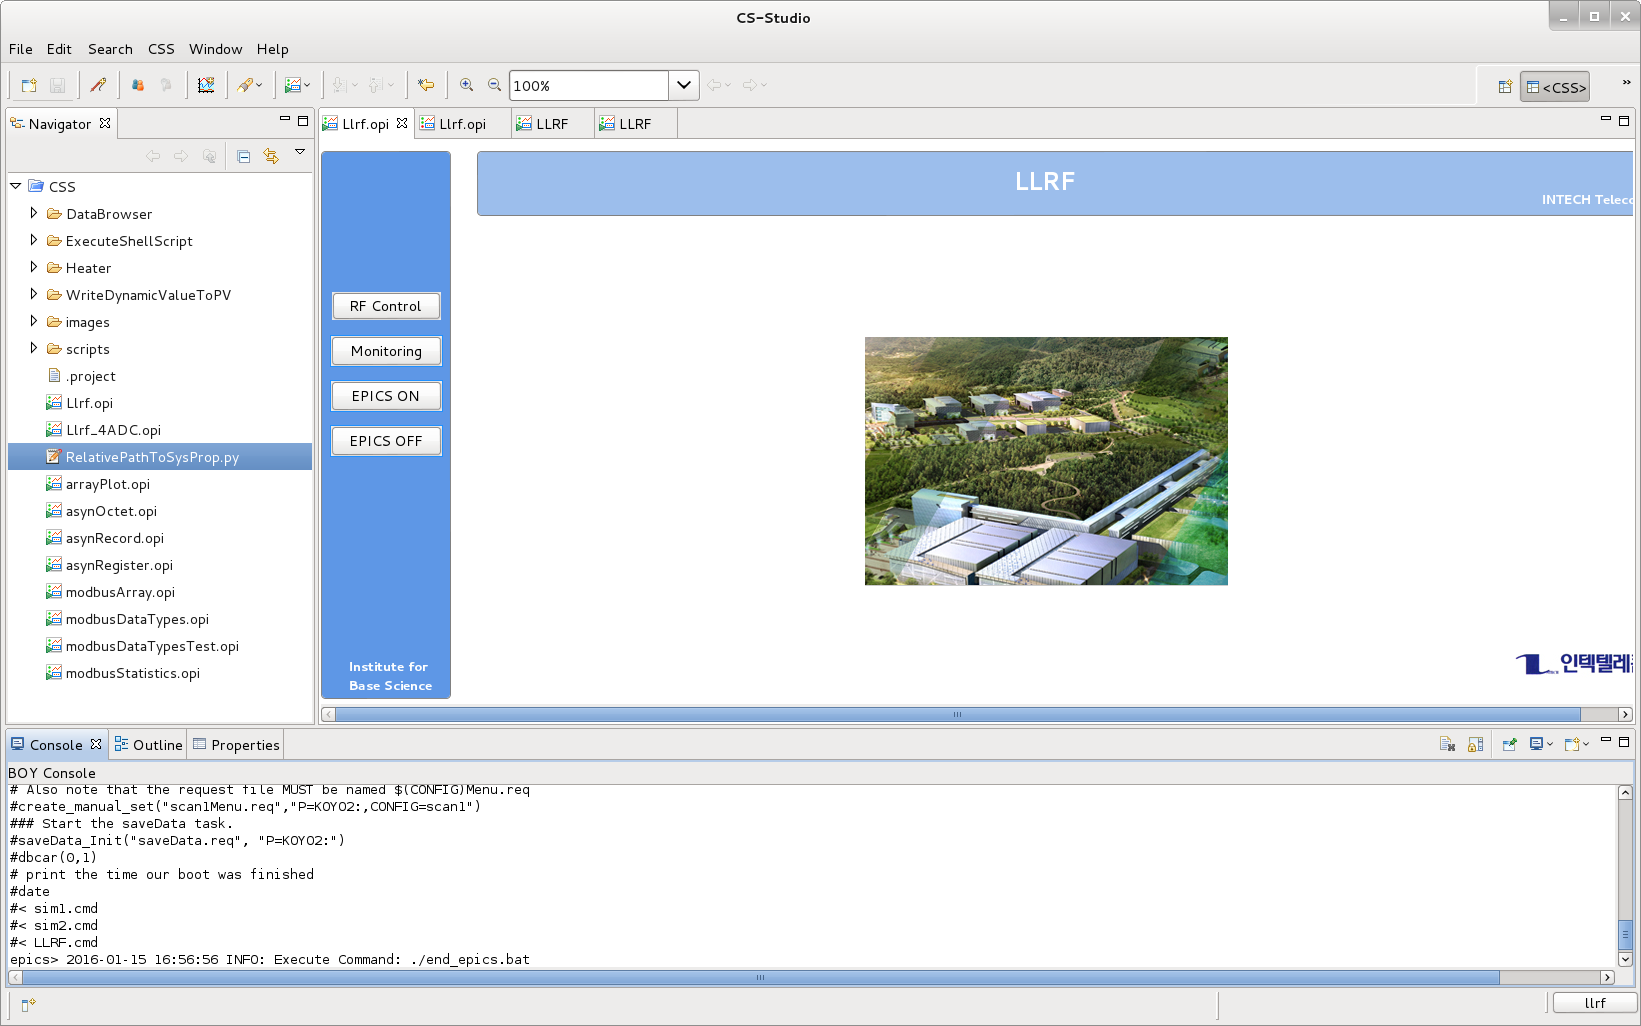
\includegraphics[width=0.85\textwidth, height=0.6\textwidth]{./images/5.png}
	\caption{CSS 실행}
\end{figure}
\begin{figure}[h!]
	\centering
	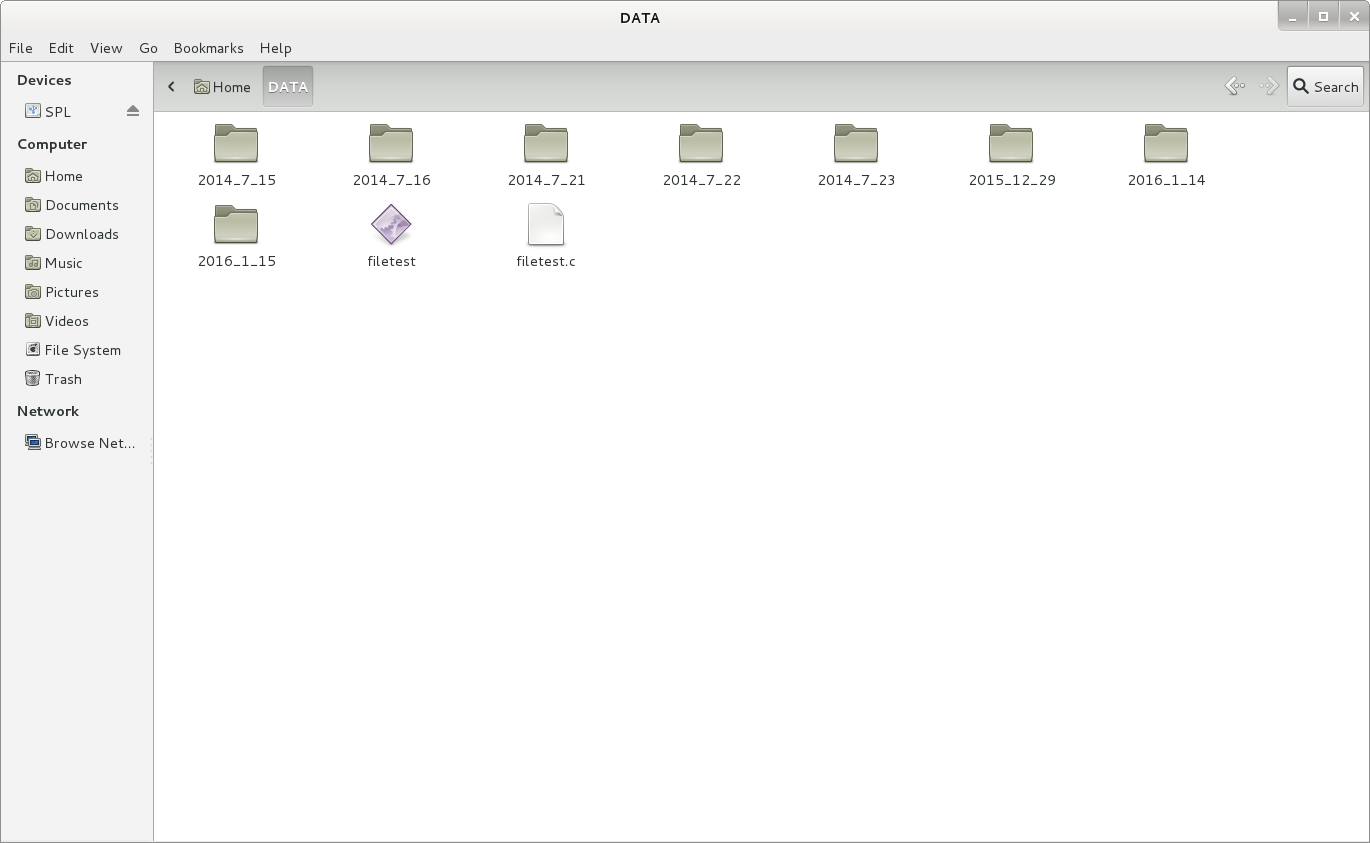
\includegraphics[width=0.85\textwidth, height=0.6\textwidth]{./images/6.png}
	\caption{PV값 저장 디렉토리}
\end{figure}
\end{document}
